%
%
%

\begin{frame}[t,allowframebreaks]{Dartmouth conference (1956) -} 

    \vspace{-0.2cm}

    \begin{columns}
        \begin{column}{0.62\textwidth}
            \begin{center}
            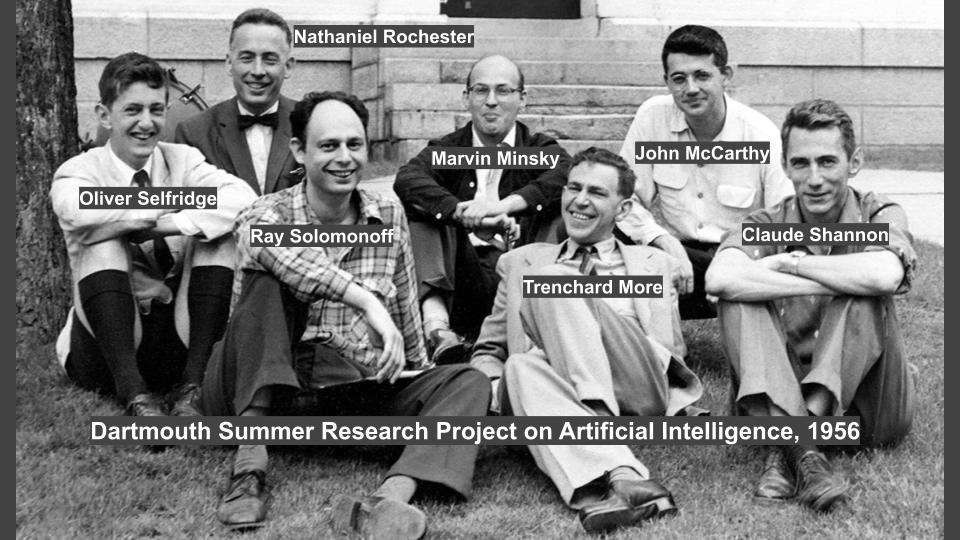
\includegraphics[width=0.98\textwidth]{./images/people/dartmouth_1956.jpg}\\
            { \scriptsize 
            \vspace{0.1cm}
            Participants in the Dartmouth Summer Research Project 
            on Artificial Intelligence, 1956.\\
            \color{col:attribution} 
            Photo labelled by Mindy McAdams
            \href{https://twitter.com/macloo/status/1319683530742431748/photo/1}{\tiny [link]}
            \\}
            \end{center}
        \end{column}
        \begin{column}{0.38\textwidth}
            \begin{blockexample}{} 
            {\tt 
                \scriptsize
                "Every aspect of learning or any other 
                feature of intelligence can in principle 
                be so precisely described that a machine can be made 
                to simulate it. An attempt will be made to find how 
                to make machines use language, form abstractions and 
                concepts, solve kinds of problems now reserved for humans, 
                and improve themselves. We think that a significant advance 
                can be made in one or more of these problems if a carefully 
                selected group of scientists work on it together for a summer."\\
            } 
           \vspace{0.2cm}
            {\scriptsize
                 A Proposal for the Dartmouth Summer Research Project 
                 on Artificial Intelligence \cite{Dartmouth:1956}.\\
            }
            \end{blockexample}
        \end{column}
    \end{columns}

    \framebreak

    \begin{blockexample}{} 
        {\tt 
            \scriptsize
            "Anybody who was there was pretty stubborn about pursuing 
            the ideas that he had before he came, nor was there, 
            as far as I could see, any real exchange of ideas."\\
            %People came for different periods of time. 
            %The idea was that everyone would agree to come for six weeks, 
            %and the people came for periods ranging from two days to 
            %the whole six weeks, so not everybody was there at once. 
            %It was a great disappointment to me because it really meant 
            %that we couldn’t have regular meetings."\\
        } 
       \vspace{0.2cm}
        {\scriptsize
             Someone \cite{Dartmouth:1956}.\\
        }
    \end{blockexample}

    \begin{blockexample}{} 
        {\tt 
            \scriptsize
            "They didn't want to hear from us, and we sure didn't want to hear 
            from them: we had something to show them! ... 
            In a way it was ironic because we already had done the first example 
            of what they were after; and second, they didn't pay much attention to it."\\
        } 
       \vspace{0.2cm}
        {\scriptsize
             H.Simon, co-creator of the Logical Theorist \cite{Crevier:1993}.\\
        }
    \end{blockexample}

    \begin{columns}
        \begin{column}{0.30\textwidth}
            \begin{center}
            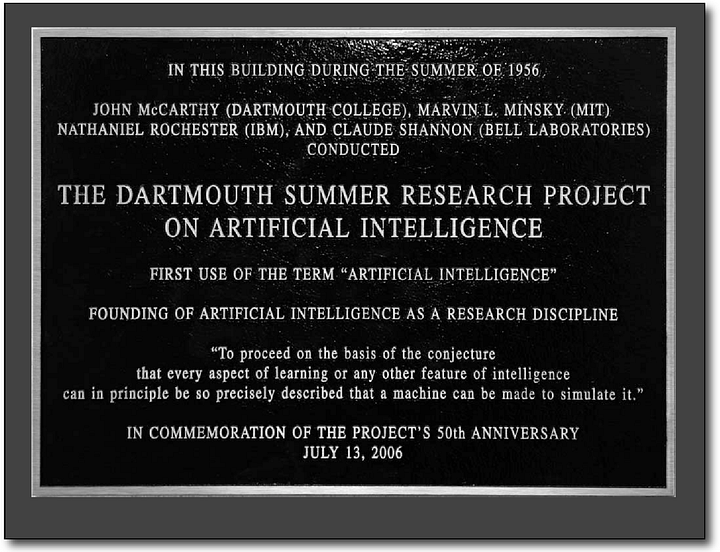
\includegraphics[width=0.98\textwidth]{./images/misc/dartmouth_commemorative_plaque.png}\\
            { \scriptsize 
            \vspace{0.1cm}
            Dartmouth Hall Commemorative Plaque..\\
            \color{col:attribution} 
            Photo by Joe Mehling, taken from \cite{Veisdal:2019dartmouth}.\\}
            \end{center}
        \end{column}
        \begin{column}{0.70\textwidth}
        \end{column}
    \end{columns}

\end{frame}